

\documentclass[10pt]{beamer}

\linespread{1.0}

\usetheme{Pittsburgh}
%\usetheme {CambridgeUS}%{Goettingen}%{Berkeley}%{Montpellier}%{Antibes}%{Dresden}%{Madrid}%{Dresden}%{Darmstadt}%{Warsaw}%{Pittsburgh}
\usefonttheme{serif}%{structurebold}%{structuresmallcapsserif}%{professionalfonts}
\usepackage[english]{babel}
%\usepackage[latin1]{inputenc}
\usepackage{hyperref}
%\usecolortheme{beaver}
%\usecolortheme{crane}

\setbeamercovered{transparent}
\newcommand{\semitransp}[2][35]{\color{fg!#1}#2}

\usepackage{latexsym}
\usepackage{amsmath}
\usepackage{times}
\usepackage{MinionPro}
\usepackage{hyperref}
\usepackage{tikz}
\usepackage{verbatim}
\usepackage{natbib}
\usepackage{color, colortbl}
\usepackage{appendix}
\usepackage{ulem}
\usepackage{amsmath,amsthm}

\usetikzlibrary{arrows,shapes}


\newtheorem{proposition}{Proposition}[section]
%\newtheorem{definition}{Definition}[section]
\newtheorem{assumption}{Assumption}[section]
\newtheorem{conjecture}{Conjecture}[section]
\newtheorem*{observation}{Observation}


\definecolor{Gray}{gray}{0.9}


\pgfdeclarelayer{background}
\pgfsetlayers{background,main}

\tikzstyle{vertex}=[circle,fill=black!25,minimum size=12pt,inner sep=0pt]
\tikzstyle{selected vertex} = [vertex, fill=red!24]
\tikzstyle{unknown vertex} = [vertex, fill=black]
\tikzstyle{edge} = [draw,thick,-]
\tikzstyle{weight} = [font=\small]
\tikzstyle{selected edge} = [draw,line width=5pt,-,red!50]
\tikzstyle{ignored edge} = [draw,line width=5pt,-,black!20]



\setbeamercovered{transparent}




\title{Coordination in Social Networks}
\author{Chun-ting Chen}


\begin{document}

\maketitle


\section{Introduction}
\subsection{Motivation}

\frame{
  \frametitle{Motivation}
  
\begin{itemize}

\item A collective action may fails due to incomplete information.
\begin{itemize}
\item A joint project, an investment, etc.
\end{itemize}
\item The situation could be severe. Eg. in pro-democracy movement 
\begin{enumerate}
\item Showing discontent is threatened by eavesdropping, suppression, etc.
\item No (fair) voting system, No (fair) mass media, No (uncensored) discussion forum, etc.


\end{enumerate} 


\end{itemize}  
  
}

\frame{
  \frametitle{Motivation}
However, history tells us:

\begin{itemize}

\item An event may trigger later events.
\begin{itemize}
\item Consecutive uprisings in East Germany 1989-1990.
\end{itemize}

\item Social networks play important role
\begin{itemize}
\item Ex., Gangster networks (1911 Revolution); Church networks (1989 Berlin Uprising), etc.
\end{itemize}



\end{itemize}  
  
}

\frame{
  \frametitle{Motivation}

Question  
  \begin{itemize}
  \item \textit{If rational rebels know that a ``tiny'' event can trigger later events, how do they conduct a decisive collective action within their social network?}
  \end{itemize}
  

Model 
\begin{enumerate}
\item No cheap talk. Communication is taking actions.
\item Communication is facing expected cost.
\item Players communicate repeatedly in a network.


\end{enumerate}





}




\frame{
  \frametitle{Motivation}

Looking for 
\begin{itemize}

\item An equilibrium, where the ex-post efficient outcome played repeatedly after a finite time $T$ in the path when $\delta$ is high enough.

\end{itemize}


}




\subsection{Literature Review}
\frame{
  \frametitle{Related Literature}

  \begin{itemize}
  \item Public good provision.
  \begin{itemize}
  \item One strand: [Chwe 2000], [Lohmann, 1993,1994], [Bolton and Harris, 1999], [Bramoull\'{e} and Kranton, 2007]
  \item \textbf{This paper adds network-monitoring}
  \end{itemize}
  \item Social learning.
  \begin{itemize}
  \item One strand: [Goyal, 2012], [Acemoglu et al., 2011], [Chatterjee and Dutta, 2011].
  \item \textbf{This paper considers farsighted-learning in the game}
  \end{itemize}
  \item Repeated game.
  \begin{itemize}
  \item One strand: [Laclau, 2012], [Wolitzky, 2013], [Wolitzky, 2014]
  \item \textbf{This paper consider incomplete information and imperfect monitoring }
  \item One strand: [Fudenberg and Yamamoto, 2010] [Fudenberg and Yamamoto, 2011] [Wiseman, 2012] [Yamamoto 2014]
  \item \textbf{This paper consider $n$-person game without full-rank conditions on public or private signals generated by single-period actions.}
  \end{itemize}
  
\end{itemize}

}



\section{Model}
\subsection{Static Game}
\frame{
  \frametitle{Model}

Network
  \begin{itemize}
  \item Let $N=\{1,...,n\}$ be the set of players. 
 
  \item $G_i$ is a subset of $N$, where $i\in G_i$
  \item $G_i$ is $i$'s neighborhood.  
  \item $G=\{G_i\}_i$ is the network.
 

 
  \end{itemize}


}


\frame{
  \frametitle{Model}


 
 \begin{definition}
 \begin{enumerate}
 \item $G$ is \textit{fixed} if $G$ is not random.
 \item $G$ is \textit{finite} if $N$ is finite.
 \item $G$ is \textit{undirected} if $j\in G_i\Rightarrow i\in G_j$.
 \item A \textit{path} from $i$ to $j$, $i\neq j$ in an undirected $G$ is 
 \[\{i,l_1,...,l_q,j\}\] 
 such that $l_1\in {G}_{i},..., l_{q}\in {G}_{j}$ and $i,l_1,...,l_q,l$ are all distinct.
 \item $G$ is \textit{connected}:  An undirected $G$ is connected $\Leftrightarrow$ $\forall$ $i,j$, $i\neq j$ there is a path from $i$ to $j$. 
 \item $G$ is \textit{acyclic}: An undirected $G$ is acyclic $\Leftrightarrow$ the path from $i$ to $j$, for $i\neq j$, is unique. 
 \end{enumerate}

\end{definition}
 


}

\frame{
  \frametitle{Model}

Static $k$-threshold game [Chwe 2000]
  \begin{itemize}
 \item $\theta_i$: $i$'s type 
 \item $\theta_i\in \Theta_i=\{Rebel,Inert\}$
  \item $\Theta=\times_{i\in N}\Theta_i$
  \item $\theta\in \Theta$
  \item $A_{Rebel_i}=\{\textbf{revolt},\textbf{stay}\}$; $A_{Inert_i}=\{\textbf{stay}\}$
  \item $1\leq k \leq n$
  \item Static game payoff for player $i$: $u_{\theta_i}(a_{\theta_i},a_{-\theta_i})$

  \begin{table}[h]
\begin{tabular}{llll}
$u_{Inert_i}(a_{Inert_i},a_{-\theta_i})$ & $=$  & 1 &  if  $a_{Inert_i}=\textbf{stay}$\\
 &  & &  \\
$u_{Rebel_i}(a_{Rebel_i},a_{-\theta_i})$ & $=$ & 1 & if $a_{Rebel_i}=\textbf{revolt}$ and $\#\{j:a_{\theta_j}=\textbf{revolt}\}\geq k$ \\
$u_{Rebel_i}(a_{Rebel_i},a_{-\theta_i})$ & $=$ & -1 & if $a_{Rebel_i}=\textbf{revolt}$ and $\#\{j:a_{\theta_j}=\textbf{revolt}\}< k$ \\
$u_{Rebel_i}(a_{Rebel_i},a_{-\theta_i})$ & $=$ & 0 & if $a_{Rebel_i}=\textbf{stay}$ \\

\end{tabular}

\end{table}
\item \textbf{stay} is a safe arm; \textbf{revolt} is a risky arm.

  \end{itemize}


}




\subsection{Repeated Game}
\begin{frame}
  \frametitle{Model}
Repeated $k$-threshold game
  \begin{itemize}

  \item  Time is infinite, discrete.
  \item Players located in $G$ at $-1$ period.
  \item Nature choose $\theta$ at $0$ period according to $\pi$.
  \item Players play the static $k$-threshold game infinitely repeatedly.


  \end{itemize}

\begin{assumption}
\begin{itemize}
\item Players know their neighbors' types.
\item Players perfectly observe their neighbors' actions. 
\item $G$ is FFCCU (fixed, finite, connected, commonly known, undirected)
  \item Payoff is hidden (or noisy, or observable).
  \item $\pi$ has full support

\item Common $\delta$. 
\end{itemize}

\end{assumption}

\end{frame}

\begin{frame}
  \frametitle{Model}

Notations:
\begin{itemize}
\item $[Rebels](\theta)=\{j:\theta_j=Rebel\}$ for all $\theta\in \Theta$.
 \item $\tau$: a strategy profile
 \item $h^{m}_{G_i}$: the history $i$ can observe up to period $m$
   \item $\beta^{\pi,\tau}_i(\theta|h^{m}_{G_i})$: $i$'s belief for a $\theta$ at period $m$. 
\end{itemize}

\end{frame}

\begin{frame}
  \frametitle{APEX}


\begin{definition}\label{Def_expost_efficient}
A sequential equilibrium is \textit{approaching ex-post efficient} (\textit{APEX}) $\Leftrightarrow$ 
\[\text{$\forall\theta$ there is a finite time $T^{\theta}$}\] 
such that ex-post efficient outcome repeats after $T^{\theta}$ in the path.
\end{definition}
 
\begin{lemma}\label{lemma_learn}
If a sequential equilibrium $\tau^*$ is APEX $\Rightarrow$
\[\text{$\forall\theta$ $\forall i$, there is a finite time $T^{\theta}_i$}\] 
such that $\sum_{\theta:\#[Rebels](\theta)\geq k}\beta^{\pi,\tau^*}_{G_i}(\theta|h^{s}_{G_i})=1$ or $=0$
if $s\geq T^{\theta}_i$.
\end{lemma}

\end{frame}



\frame{
  \frametitle{Leading Example}

An Apex Equilibrium for $k=n=3$ in
  \begin{center}
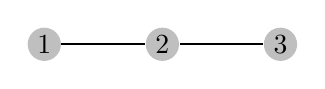
\begin{tikzpicture}[scale=1.5]
    % Draw a 7,11 network
    % First we draw the vertices
    \foreach \pos/\name in {{(1,0)/1}, {(2,0)/2}, {(3,0)/3}}
        \node[vertex] (\name) at \pos {$\name$};
    % Connect vertices with edges 
    \foreach \source/ \dest in {1/2, 2/3}
        \path[edge] (\source) -- (\dest) ;
        
\end{tikzpicture}
\end{center}

\begin{itemize}
\item At 1st period
\begin{itemize}
\item Rebel 2 chooses $\textbf{revolt}$ if he observes $\theta=(Rebel,Rebel,Rebel)$; Otherwise, chooses $\textbf{stay}$ forever.
\item Rebel 1 (or Rebel 3) choose \textbf{stay}.
\end{itemize}

\item After 1st period
\begin{itemize}
\item If Rebel 2 chooses \textbf{revolt} in the last period, then Rebel 1 (or Rebel 3) chooses \textbf{revolt} forever; 
\item If Rebel 2 chooses \textbf{stay} in the last period, then Rebel 1 (or Rebel 3) chooses \textbf{stay} forever.
\end{itemize}
 
 \item Any deviation $\Rightarrow$
 \begin{itemize}
 \item Choosing \textbf{stay} forever.
 \end{itemize}
\end{itemize}

  
}


\frame{
  \frametitle{Goal}

\textbf{Goal}

Can we generalize the above result for all FFCCU networks?



}

\frame{
  \frametitle{Results}

\textbf{Results}
\begin{itemize}
\item $k=n$: we can.
\item $k<n$: with additional assumption,
\begin{itemize}
\item acyclic networks: we can .
\item all networks: open question.
\end{itemize}
\end{itemize}

}


\frame{
  \frametitle{Result: $k=n$}

\begin{theorem}

\textbf{In} any FFCCU network, \textbf{if}  the prior has full support, \textbf{then} for repeated $k=n$ Threshold game, \textbf{there is} a $\delta$ such that a sequential equilibrium which is APEX \textbf{exists}.
\end{theorem}

Proof:
  \begin{enumerate}
  

  \item Some Inerts neighbors $\Rightarrow$ play \textbf{stay} forever.
  \item No Inert neighbor $\Rightarrow$ play \textbf{revolt} until \textbf{stay} is observed, and then play \textbf{stay} forever.
  \item Any deviation $\Rightarrow$ play \textbf{stay} forever.
  \item Since networks are FFCCU, there is a finite time $T^{\theta}$ such that ex-post efficient outcome repeats afterwards.

   \end{enumerate}

}

\frame{
  \frametitle{Result: $k=n$}

Comments:
\begin{enumerate}
\item \textbf{stay} means  ``some Inerts are out there.''
\item \textbf{revolt} means ``some Inerts may not be there.''
\item Any deviation $\Rightarrow$ punished by shifting to \textbf{stay} forever by single player
\begin{itemize}
\item Group punishment is not necessary.
\end{itemize}
\end{enumerate}
}


\begin{frame}
  \frametitle{Result and Conjecture: $k<n$}


\begin{definition}
\textbf{Strong connectedness}$\Leftrightarrow$ for every pair of Rebels, there is a path consisting of Rebels to connect them.
\end{definition}  

\begin{definition}
\textbf{Full support on strong connectedness}$\Leftrightarrow$ 
\[\text{$\pi(\theta)>0$ if and only if $\theta$ has strong connectedness.}\]


\end{definition}  

\end{frame}





\begin{frame}
  \frametitle{Result and Conjecture: $k<n$}



\begin{theorem}
\label{thm_main_result}
\textbf{In} any {acyclic} FFCCU network, \textbf{if} $\pi$ has full support  {on strong connectedness}, \textbf{then} for repeated $1\leq k \leq n$ Threshold game, \textbf{there is} a $\delta$ such that a {weak} sequential equilibrium which is APEX \textbf{exists}.
\end{theorem}

\begin{conjecture}
\textbf{In} any FFCCU network, ...[same as above]...
\end{conjecture}

\end{frame}

\section{Equilibrium construction}
\subsection{Equilibrium construction}

\frame{
  \frametitle{Equilibrium Construction: $k<n$}
\framesubtitle{Outline}

Outline

\begin{enumerate}
\item The role of Strong Connectedness
\item Communication by actions
\item Communication in the equilibrium
\begin{enumerate}
\item Communication protocol
\item Reporting and coordination messages in the protocol
\item Information hierarchy in communication
\item In-the-path belief updating
\item Off-path belief
\item Sketch of proof
\end{enumerate}

\end{enumerate}

}



\begin{frame}
   \frametitle{The role of Strong Connectedness}


\textbf{The role of Strong Connectedness}: 
\begin{itemize}
\item Otherwise, APEX is impossible for some $k$.
\end{itemize}

\begin{enumerate}


\item Let $k=2$. 
\item Let 
\begin{center}
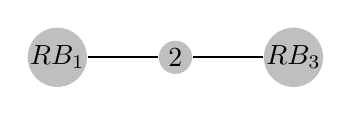
\begin{tikzpicture}[scale=1.5]
    % Draw a 7,11 network
    % First we draw the vertices
    \foreach \pos/\name in {{(1,0)/RB_1}, {(2,0)/2}, {(3,0)/RB_3}}
        \node[vertex] (\name) at \pos {$\name$};
    % Connect vertices with edges 
    \foreach \source/ \dest in {RB_1/2, 2/RB_3}
        \path[edge] (\source) -- (\dest) ;
        
\end{tikzpicture}
\end{center}
\item Inert 2 block the information transmission.
\item This is an incomplete information game without communication.





\end{enumerate}
 




\end{frame}


\begin{frame}
  \frametitle{Communication by actions}

\textbf{Communication by binary actions}
\begin{enumerate}


\item Indexing each node $i$ as a distinct prime number $x_i$. For instance,
\begin{center} 
  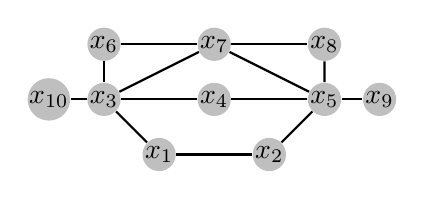
\begin{tikzpicture}[scale=0.7]
    % First we draw the vertices
    \foreach \pos/\name in {{(2,1)/x_1}, {(4,1)/x_2}, {(1,2)/x_3}, {(5,2)/x_5}, {(3,3)/x_7}, {(3,2)/x_4}, {(1,3)/x_6}, {(5,3)/x_8}, {(6,2)/x_9}, {(0,2)/x_{10}}}
        \node[vertex] (\name) at \pos {$\name$};
        
%        \foreach \pos/\name in {{(3,2)/4_L}, {(1,3)/6_L}, {(5,3)/8_L}, {(6,2)/9_L}, {(0,2)/10_L}}
%   \node[selected vertex] (\name) at \pos {$\name$};
    
    % Connect vertices with edges 
    \foreach \source/ \dest in {x_1/x_2, x_1/x_3, x_2/x_5, x_3/x_4, x_3/x_6, x_3/x_7, x_4/x_5, x_5/x_7, x_5/x_8, x_5/x_9,x_6/x_7, x_7/x_8, x_3/x_{10}}
        \path[edge] (\source) -- (\dest) ;
\end{tikzpicture}
\end{center} 
\item Then,  If
\begin{center} 
  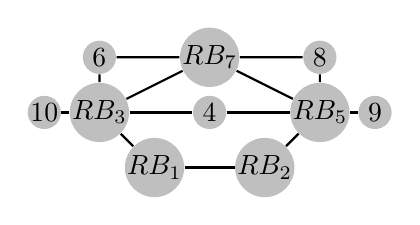
\begin{tikzpicture}[scale=0.7]
    % First we draw the vertices
    \foreach \pos/\name in {{(2,1)/RB_1}, {(4,1)/RB_2}, {(1,2)/RB_3}, {(5,2)/RB_5}, {(3,3)/RB_7}, {(3,2)/4}, {(1,3)/6}, {(5,3)/8}, {(6,2)/9}, {(0,2)/10}}
        \node[vertex] (\name) at \pos {$\name$};
        
%        \foreach \pos/\name in {{(3,2)/4_L}, {(1,3)/6_L}, {(5,3)/8_L}, {(6,2)/9_L}, {(0,2)/10_L}}
%   \node[selected vertex] (\name) at \pos {$\name$};
    
    % Connect vertices with edges 
    \foreach \source/ \dest in {RB_1/RB_2, RB_1/RB_3, RB_2/RB_5, RB_3/4, RB_3/6, RB_3/RB_7, 4/RB_5, RB_5/RB_7, RB_5/8, RB_5/9,6/RB_7, RB_7/8, RB_3/10}
        \path[edge] (\source) -- (\dest) ;
\end{tikzpicture}
\end{center} 

Rebel 3 report $x_1\times x_7 \times x_3$ to Rebel 1 by sending a finite sequence 
\[\textbf{stay},...,\textbf{stay},\underbrace{\textbf{revolt},\textbf{stay},...,\textbf{stay}}_{x_1\times x_7 \times x_3}\]

\end{enumerate}


\end{frame}









\begin{frame}
  \frametitle{Communication protocol}

\textbf{Communication phase}

Characterize the time horizontal line as 
\[\underbrace{\langle\text{coordination period}\rangle}_{0-block}\underbrace{\langle\text{reporting period}\rangle \langle\text{coordination period}\rangle}_{1-block}...\]

\begin{itemize}
\item \alert{Reporting period}: talking about $\theta$
\begin{itemize}
\item Cheap talking: $\theta$ will be revealed.
\end{itemize}
\item Why do I need \alert{coordination period} ?


\end{itemize}


\end{frame}


\begin{frame}
  \frametitle{Communication protocol}

\textbf{Coordination period}

Why do I need coordination period ?
\begin{itemize}
\item Ans: Since higher-order belief is hard to track.

\begin{itemize}
\item APEX: to find $T^{\theta}$ for all $\theta$.
\item When is $T^{\theta}$?.
\end{itemize}
\item Sol: Let $CD$ be long enough in a block

\[\overbrace{\langle ... \rangle}^{\text{RP}}\overbrace{\langle \langle \cdot \rangle \langle \cdot \rangle...\langle \cdot \rangle\rangle}^{\text{CD}}\] 
\invisible{\begin{itemize}
\item If a Rebel knows relevant info., $\Rightarrow$ sending messages to let neighbors know $\Rightarrow$ neighbors send msg. to let their neighbors know $\Rightarrow$....
\end{itemize}}

\end{itemize}

\end{frame}

\begin{frame}
  \frametitle{Communication protocol}

\textbf{Coordination period}

Why do I need coordination period ?
\begin{itemize}
\item Ans: Since higher-order belief is hard to track.

\begin{itemize}
\item APEX: to find $T^{\theta}$ for all $\theta$.
\item When is $T^{\theta}$?.
\end{itemize}
\item Sol: Let $CD$ be long enough in a block

\[\overbrace{\alert{\langle ... \rangle}}^{RP}\overbrace{\langle \langle \cdot \rangle \langle \cdot \rangle...\langle \cdot \rangle\rangle}^{CD}\] 
\begin{itemize}
\item If a Rebel knows the relevant info. after $RP$, \invisible{$\Rightarrow$ sending messages to let neighbors know $\Rightarrow$ neighbors send msg. to let their neighbors know $\Rightarrow$....}
\end{itemize}

\end{itemize}

\end{frame}




\begin{frame}
  \frametitle{Communication protocol}

\textbf{Coordination period}

Why do I need coordination period ?
\begin{itemize}
\item Ans: Since higher-order belief is hard to track.

\begin{itemize}
\item APEX: to find $T^{\theta}$ for all $\theta$.
\item When is $T^{\theta}$?.
\end{itemize}
\item Sol: Let $CD$ be long enough in a block

\[\overbrace{\alert{\langle ... \rangle}}^{RP}\overbrace{\langle \alert{\langle \cdot \rangle} \langle \cdot \rangle...\langle \cdot \rangle\rangle}^{CD}\] 
\begin{itemize}
\item If a Rebel knows the relevant info. after $RP$,$\Rightarrow$ sending messages to let neighbors know that \invisible{$\Rightarrow$ neighbors send msg. to let their neighbors know $\Rightarrow$....$\Rightarrow$ all the Rebels know that.}
\end{itemize}

\end{itemize}

\end{frame}

\begin{frame}
  \frametitle{Communication protocol}

\textbf{Coordination period}

Why do I need coordination period ?
\begin{itemize}
\item Ans: Since higher-order belief is hard to track.

\begin{itemize}
\item APEX: to find $T^{\theta}$ for all $\theta$.
\item When is $T^{\theta}$?.
\end{itemize}
\item Sol: Let $CD$ be long enough in a block

\[\overbrace{\alert{\langle ... \rangle}}^{RP}\overbrace{\langle \alert{\langle \cdot \rangle \langle \cdot \rangle...\langle \cdot \rangle}\rangle}^{CD}\] 
\begin{itemize}
\item If a Rebel knows the relevant info. after $RP$ $\Rightarrow$ sending messages to let neighbors know that {$\Rightarrow$ neighbors send msg. to let their neighbors know $\Rightarrow$....$\Rightarrow$ \alert{all the Rebels commonly know that after this block}.}
\end{itemize}

\end{itemize}

\end{frame}


\begin{frame}
\frametitle{Communication protocol}

\textbf{After coordination period}

\begin{itemize}
\item Either stopping or continuing communication
\begin{enumerate}
\item \alert{Stopping}: if relevant info. is revealed $\Rightarrow$ messages will be sent $\Rightarrow$ all Rebels play the ex-post eff. outcome afterward. 
\item \alert{Continuing}: otherwise, go to the next block.
\end{enumerate}

\end{itemize}

\begin{observation}
This protocol will let Rebels either stop or continue updating their information about $\theta$ after a block.
\end{observation}

$\Rightarrow$ a \alert{protocol-grim-trigger}. 
\end{frame}


\begin{frame}
\frametitle{Equilibrium path}

\textbf{Coordination period and messages}

Idea
\begin{itemize}
\item At least ``\alert{three}'' messages to coordinate Rebels
\begin{enumerate}
\item to \textbf{revolt}
\item to \textbf{stay}
\item to continue to next block 
\end{enumerate}
\item Create these \alert{distinguishable} messages by binary actions
\end{itemize}



\end{frame}


\begin{frame}
\frametitle{Equilibrium path}

\textbf{Coordination period and messages}

\begin{itemize}
\item $CD^t$: the $CD$ in $t$-block

\[\overbrace{\langle\underbrace{\langle \cdot \rangle \cdot \cdot \cdot \langle \cdot \rangle}_{\text{1st division}}\rangle \langle\underbrace{\langle \cdot \rangle \cdot \cdot \cdot \langle \cdot \rangle}_{\text{2nd division}} \rangle }^{CD^t}\] 
\item $CD^t_{p,q}$: the $p$ sub-block in $q$ division.
\item $\langle CD^t_{p,q} \rangle$: the messages in $CD^t_{p,q}$ are \alert{distinguishable}
\begin{table}[h]
\begin{tabular}{l l}
$\langle \textbf{stay} \rangle$ & $\textbf{s},...,\textbf{s},\textbf{s},\textbf{s},...,\textbf{s}$  \\
$\langle x_i\rangle$ & $\textbf{s},...,\textbf{s},\underbrace{\textbf{r},\textbf{s},...,\textbf{s}}_{x_i}$ \\
\end{tabular}
\end{table}
\item 1st division: sending \textbf{message to stay}; otherwise \textbf{continue}
\item 2nd division: sending \textbf{message to revolt}; otherwise \textbf{continue}
\end{itemize}



\end{frame}

\begin{frame}
\frametitle{Equilibrium path}

\textbf{Message to \textbf{stay}}

\begin{itemize}
\item Whenever a Rebel $i$ knows \alert{$\#[Rebels](\theta)<k$} 

\[\overbrace{\langle\underbrace{\alert{\langle \textbf{stay} \rangle} \langle \cdot \rangle ... \langle \cdot \rangle}_{\text{1st division}}\rangle \langle\underbrace{\langle \cdot \rangle \cdot \cdot \cdot \langle \cdot \rangle}_{\text{2nd division}} \rangle }^{CD^t}\] 
\item \alert{Otherwise} ,

\[\overbrace{\langle\underbrace{\alert{\langle x_i \rangle} \langle \cdot \rangle ... \langle \cdot \rangle}_{\text{1st division}}\rangle \langle\underbrace{\langle \cdot \rangle \cdot \cdot \cdot \langle \cdot \rangle}_{\text{2nd division}} \rangle }^{CD^t}\] 

\end{itemize}

\end{frame}

\begin{frame}
\frametitle{Equilibrium path}

\textbf{Message to \textbf{stay}}

\begin{itemize}
\item Then nearby Rebel $j$ \alert{play \textbf{stay} afterward}
\[\overbrace{\langle\underbrace{\alert{\langle x_i \rangle} \alert{\langle \textbf{stay} \rangle} ... \langle \cdot \rangle}_{\text{1st division}}\rangle \langle\underbrace{\langle \cdot \rangle \cdot \cdot \cdot \langle \cdot \rangle}_{\text{2nd division}} \rangle }^{CD^t}\] 

\item \alert{Otherwise},
\[\overbrace{\langle\underbrace{\alert{\langle x_i \rangle} \alert{\langle x_i \rangle} ... \langle \cdot \rangle}_{\text{1st division}}\rangle \langle\underbrace{\langle \cdot \rangle \cdot \cdot \cdot \langle \cdot \rangle}_{\text{2nd division}} \rangle }^{CD^t}\] 

\end{itemize}

\end{frame}


\begin{frame}
\frametitle{Equilibrium path}

\textbf{Message to \textbf{revolt}}

\begin{itemize}
\item Whenever a Rebel $i$ know \alert{$\#[Rebels](\theta)\geq k$}

\[\overbrace{\langle\underbrace{\langle \cdot \rangle \cdot \cdot \cdot \langle \cdot \rangle}_{\text{1st division}}\rangle \langle\underbrace{\alert{\langle \textbf{stay} \rangle} \langle \cdot \rangle \cdot \cdot \langle \cdot \rangle}_{\text{2nd division}} \rangle }^{CD^t}\] 

\item \alert{Otherwise} ,
\[\overbrace{\langle\underbrace{\langle \cdot \rangle \cdot \cdot \cdot \langle \cdot \rangle}_{\text{1st division}}\rangle \langle\underbrace{\alert{\langle x_i \rangle} \langle \cdot \rangle \cdot \cdot \langle \cdot \rangle}_{\text{2nd division}} \rangle }^{CD^t}\]
\end{itemize}

\end{frame}


\begin{frame}
\frametitle{Equilibrium path}

\textbf{Message to \textbf{revolt}}

\begin{itemize}
\item Then nearby Rebel $j$ \alert{play $\langle x_j \rangle$ to inform nearby Rebels, etc}

\[\overbrace{\langle\underbrace{\langle \cdot \rangle \cdot \cdot \cdot \langle \cdot \rangle}_{\text{1st division}}\rangle \langle\underbrace{\alert{\langle x_j \rangle} \alert{\langle x_j \rangle} \cdot \cdot \langle \cdot \rangle}_{\text{2nd division}} \rangle }^{CD^t}\] 

\item \alert{Otherwise} ,

\[\overbrace{\langle\underbrace{\langle \cdot \rangle \cdot \cdot \cdot \langle \cdot \rangle}_{\text{1st division}}\rangle \langle\underbrace{\alert{\langle x_j \rangle} \alert{\langle \textbf{stay} \rangle} \cdot \cdot \langle \cdot \rangle}_{\text{2nd division}} \rangle }^{CD^t}\] 

\end{itemize}

\end{frame}


\begin{frame}
\frametitle{Equilibrium path}

\textbf{Coordination messages}

\begin{itemize}
\item \alert{No expected cost} to send \textbf{Message to stay} in $CD^t_{1,1}$ or \textbf{Message to revolt} in $CD^t_{1,2}$
\begin{itemize}
\item Both are $\langle \textbf{stay}\rangle$
\end{itemize}


\item In this protocol, if $\delta$ is high enough then
\begin{lemma}
Before a Rebel knows $\#[Rebels](\theta)< k$ or $\#[Rebels](\theta)\geq k$ , he will not send \textbf{Message to stay} or \textbf{Message to revolt}.
\end{lemma}
\begin{enumerate}
\item Ex-post efficient outcome gives the maximum static ex-post payoff.
\item protocol-grim-trigger: information updating stops after $CD^t_{1,1}=\langle \textbf{stay} \rangle$ or $CD^t_{1,2}=\langle \textbf{stay} \rangle$.
\item So, he is better not to send those messages..  
\end{enumerate}


\end{itemize}

\end{frame}


\begin{frame}
\frametitle{Equilibrium path}

\textbf{Reporting period and messages}

Idea

\begin{itemize}
\item ``{Burning moneys}'' before sending \textbf{message to revolt}.
\begin{enumerate}
\item Gives incentives to report $\theta$.
\item Prevent potential free rider problems.
\end{enumerate}
\item Characterizing ``how much money a Rebel should burn'' 
\begin{itemize}
\item Building Information Hierarchy
\end{itemize}

\end{itemize}

\end{frame}


\begin{frame}
\frametitle{Equilibrium path}

\textbf{Reporting period and messages}

\begin{itemize}
\item $RP^t$: the reporting period at $t$ block

\[\overbrace{\langle \langle \cdot \rangle \rangle}^{RP^t}\] 

\item $\langle RP^t \rangle$: the reporting message
\begin{table}[h]
\begin{tabular}{l l l}
\alert{Burning moneys} & $\neg\langle \textbf{stay} \rangle$ & $\textbf{s},...,\textbf{s},{\textbf{r},\textbf{s},...,\textbf{s}}$ \\
\hline
\alert{Not burning money} & $\langle \textbf{stay} \rangle$ & $\textbf{s},...,\textbf{s},\textbf{s},\textbf{s},...,\textbf{s}$  \\

\end{tabular}
\end{table}
\item \alert{Burning moneys}+\textbf{message to revolt}: 
\begin{itemize}
\item Rebels believe that $\#[Rebels](\theta)\geq k$
\end{itemize}

\item \alert{Not burning moneys}+\textbf{message to revolt}: 

\begin{itemize}
\item Rebels don't believe that $\#[Rebels](\theta)\geq k$
\end{itemize}

\end{itemize}
\end{frame}


\begin{frame}
\frametitle{Equilibrium path}

\textbf{An example for free rider problem if no money burning}

Assume,
\begin{enumerate}
\item Only one block.
\item No expected cost in $CD$.
\item Obs. $\langle M \rangle$ in $CD$ $\Rightarrow$ play \textbf{revolt} forever; 
\item Obs. $\neg \langle M \rangle$ in $CD$ $\Rightarrow$ play \textbf{stay} forever.
\item $k=5$
\item Free riders:
\begin{center}
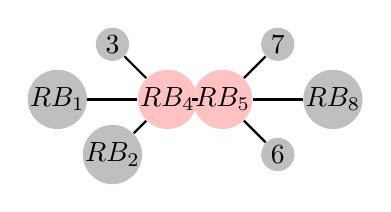
\begin{tikzpicture}[scale=0.7]
    % Draw a 7,11 network
    % First we draw the vertices
    \foreach \pos/\name in {{(1,2)/RB_1}, {(2,1)/RB_2}, {(2,3)/3}, {(5,1)/6}, {(5,3)/7}, {(6,2)/RB_8}}
        \node[vertex] (\name) at \pos {$\name$};
    
    \foreach \pos/\name in {{(3,2)/RB_4}, {(4,2)/RB_5}}
    \node[selected vertex] (\name) at \pos {$\name$};
    
    % Connect vertices with edges 
    \foreach \source/ \dest in {RB_1/RB_4, RB_2/RB_4,3/RB_4,RB_4/RB_5, RB_5/6, RB_5/7, RB_5/RB_8}
        \path[edge] (\source) -- (\dest) ;
        
\end{tikzpicture}
\end{center}

\item Rebel 4 will not burn money if Rebel 5 report truthfully, and vise versa.

\end{enumerate}

\begin{observation}
\begin{enumerate}
\item Some Rebels \alert{will} know $\#[Rebels](\theta)\geq k$ or $\#[Rebels](\theta)< k$ after $RP$.
\item The ``meaning'' of $\langle M \rangle$ or $\neg \langle M \rangle$ should not be free from burning money.
\end{enumerate}
\end{observation}

\end{frame}


\begin{frame}
\frametitle{Equilibrium path}

\textbf{How much money should a Rebel burns?}

\begin{itemize}
\item Burning money is to convince Rebels to {coordination to revolt}.
\item \alert{Information Hierarchy}: how much money should be burned?.
\end{itemize}

\end{frame}


\begin{frame}
   \frametitle{Information Hierarchy}


Main goal of \textbf{Information Hierarchy}
\begin{itemize}
\item Characterizing Rebels' incentives in money burning.
\item Ex: $k=4$ and
\begin{center}
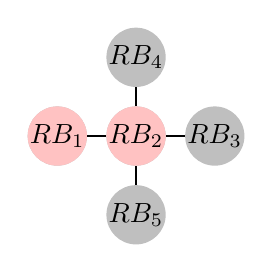
\begin{tikzpicture}[scale=1]
    % Draw a 7,11 network
    % First we draw the vertices
    \foreach \pos/\name in {{(1,1)/RB_1}, {(2,1)/RB_2}, {(3,1)/RB_3}, {(2,2)/RB_4}, {(2,0)/RB_5}}
        \node[vertex] (\name) at \pos {$\name$};
        
    \foreach \pos/\name in {{(1,1)/RB_1}, {(2,1)/RB_2}}
    \node[selected vertex] (\name) at \pos {$\name$};
    % Connect vertices with edges 
    \foreach \source/ \dest in {RB_1/RB_2, RB_2/RB_3, RB_4/RB_2, RB_2/RB_5}
        \path[edge] (\source) -- (\dest) ;
        
\end{tikzpicture}
\end{center}

\begin{enumerate}
\item Rebel 1's information can be reported by Rebel 2.
\end{enumerate}

\end{itemize}



\end{frame}

\begin{frame}
   \frametitle{Information Hierarchy}


Main goal of \textbf{Information Hierarchy}
\begin{itemize}
\item Easing the punishment scheme when monitoring is imperfect.
\item Note that $k<n$, punishment by single player is not enough.
\item Ex: $k=4$ and
\begin{center}
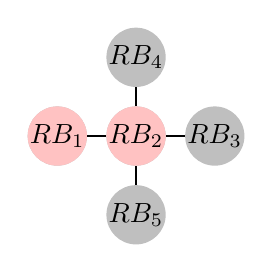
\begin{tikzpicture}[scale=1]
    % Draw a 7,11 network
    % First we draw the vertices
    \foreach \pos/\name in {{(1,1)/RB_1}, {(2,1)/RB_2}, {(3,1)/RB_3}, {(2,2)/RB_4}, {(2,0)/RB_5}}
        \node[vertex] (\name) at \pos {$\name$};
        
    \foreach \pos/\name in {{(1,1)/RB_1}, {(2,1)/RB_2}}
    \node[selected vertex] (\name) at \pos {$\name$};
    % Connect vertices with edges 
    \foreach \source/ \dest in {RB_1/RB_2, RB_2/RB_3, RB_4/RB_2, RB_2/RB_5}
        \path[edge] (\source) -- (\dest) ;
        
\end{tikzpicture}
\end{center}

\begin{enumerate}
\item Rebel 1 can only be monitored by Rebel 2.
\item Suppose Rebel 2,3,4,5 can coordinate at period $T$ and play \textbf{revolt} forever.
\item If Rebel 1 did not burn money at period $T-1$, Rebel 2 has no incentive to punish him.
\end{enumerate}

\end{itemize}



\end{frame}














\begin{frame}
  \frametitle{Information Hierarchy}

\textbf{Information Hierarchy}  
  
\begin{center}
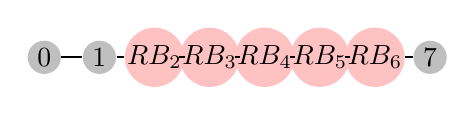
\begin{tikzpicture}[scale=0.7]
    % Draw a 7,11 network
    % First we draw the vertices
    \foreach \pos/\name in {{(0,1)/1},{(6,1)/7},{(-1,1)/0}}
        \node[vertex] (\name) at \pos {$\name$};
        
    \foreach \pos/\name in {{(1,1)/RB_2}, {(2,1)/RB_3}, {(3,1)/RB_4}, {(4,1)/RB_5}, {(5,1)/RB_6}}
    \node[selected vertex] (\name) at \pos {$\name$};
    
    % Connect vertices with edges 
    \foreach \source/ \dest in {1/RB_2,RB_2/RB_3, RB_3/RB_4, RB_4/RB_5, RB_5/RB_6,RB_6/7,0/1}
        \path[edge] (\source) -- (\dest) ;
        
\end{tikzpicture}
\end{center}


At $\alert{0}$-block, let

 \[\alert{R^0}=[Rebels](\theta)\]



\end{frame}

\begin{frame}
  \frametitle{Information Hierarchy}
 

\begin{center}
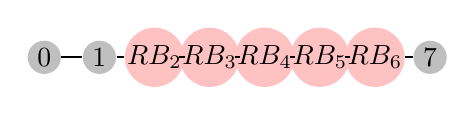
\begin{tikzpicture}[scale=0.7]
    % Draw a 7,11 network
    % First we draw the vertices
    \foreach \pos/\name in {{(0,1)/1},{(6,1)/7},{(-1,1)/0}}
        \node[vertex] (\name) at \pos {$\name$};
        
    \foreach \pos/\name in {{(1,1)/RB_2}, {(2,1)/RB_3}, {(3,1)/RB_4}, {(4,1)/RB_5}, {(5,1)/RB_6}}
    \node[selected vertex] (\name) at \pos {$\name$};
    
    % Connect vertices with edges 
    \foreach \source/ \dest in {1/RB_2,RB_2/RB_3, RB_3/RB_4, RB_4/RB_5, RB_5/RB_6,RB_6/7,0/1}
        \path[edge] (\source) -- (\dest) ;
        
\end{tikzpicture}
\end{center}

At $1$-block, first let
\begin{eqnarray*}
G^0_i & \equiv &  G_i\\
I^0_i & \equiv & G_i\cap R^0\\
\end{eqnarray*}

For instance,
\begin{table}[h]
\begin{tabular}{l l}
$I^0_2=\{2,3\} $ &  $G^0_2=\{1,2,3\}$  \\
$I^0_3=\{2,3,4\}$ & $G^0_3=\{2,3,4\} $  
\end{tabular}
\end{table}

\end{frame}


\begin{frame}
  \frametitle{Information Hierarchy}


\begin{center}
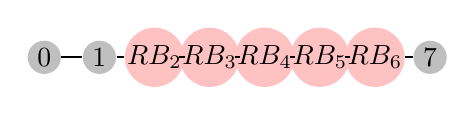
\begin{tikzpicture}[scale=0.7]
    % Draw a 7,11 network
    % First we draw the vertices
    \foreach \pos/\name in {{(0,1)/1},{(6,1)/7},{(-1,1)/0}}
        \node[vertex] (\name) at \pos {$\name$};
        
    \foreach \pos/\name in {{(1,1)/RB_2}, {(2,1)/RB_3}, {(3,1)/RB_4}, {(4,1)/RB_5}, {(5,1)/RB_6}}
    \node[selected vertex] (\name) at \pos {$\name$};
    
    % Connect vertices with edges 
    \foreach \source/ \dest in {1/RB_2,RB_2/RB_3, RB_3/RB_4, RB_4/RB_5, RB_5/RB_6,RB_6/7,0/1}
        \path[edge] (\source) -- (\dest) ;
        
\end{tikzpicture}
\end{center}

Then define \[\leq^0\] by
\[i\in \leq^0 \Leftrightarrow \exists  j\in \bar{G}_i (I^0_i\subseteq G^0_j\cap R^0)\] 

\begin{itemize}
\item For instance, \[2\in \leq^0, 3\notin \leq^0\]
\item Since \begin{table}[h]
\begin{tabular}{l l}
$I^0_2=\{2,3\} $ &  {$G^0_2\cap R^0=\{2,3\}$}  \\
{$I^0_3=\{2,3,4\}$} & $G^0_3\cap R^0=\{2,3,4\} $ 
\end{tabular}
\end{table}
\end{itemize}




\end{frame}




\begin{frame}
  \frametitle{Information Hierarchy}


\begin{center}
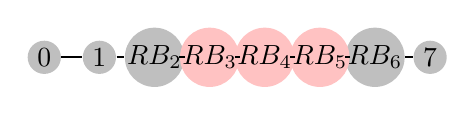
\begin{tikzpicture}[scale=0.7]
    % Draw a 7,11 network
    % First we draw the vertices
    \foreach \pos/\name in {{(0,1)/1},{(6,1)/7},{(1,1)/RB_2},{(5,1)/RB_6},{(-1,1)/0}}
        \node[vertex] (\name) at \pos {$\name$};
        
    \foreach \pos/\name in {{(2,1)/RB_3}, {(3,1)/RB_4}, {(4,1)/RB_5}}
    \node[selected vertex] (\name) at \pos {$\name$};
    
    % Connect vertices with edges 
    \foreach \source/ \dest in {1/RB_2,RB_2/RB_3, RB_3/RB_4, RB_4/RB_5, RB_5/RB_6,RB_6/7,0/1}
        \path[edge] (\source) -- (\dest) ;
        
\end{tikzpicture}
\end{center}

At $\alert{1}$-block, let

\[
\alert{R^{1}} \equiv \{i\in R^0|i\notin \leq^0\}=\{\invisible{2,}3,4,5\invisible{,6}\}
\]




\end{frame}

\begin{frame}
  \frametitle{Information Hierarchy}


\begin{center}
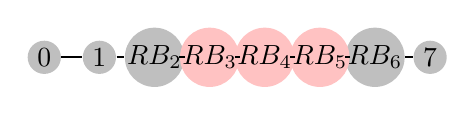
\begin{tikzpicture}[scale=0.7]
    % Draw a 7,11 network
    % First we draw the vertices
    \foreach \pos/\name in {{(0,1)/1},{(6,1)/7},{(1,1)/RB_2},{(5,1)/RB_6},{(-1,1)/0}}
        \node[vertex] (\name) at \pos {$\name$};
        
    \foreach \pos/\name in {{(2,1)/RB_3}, {(3,1)/RB_4}, {(4,1)/RB_5}}
    \node[selected vertex] (\name) at \pos {$\name$};
    
    % Connect vertices with edges 
    \foreach \source/ \dest in {1/RB_2,RB_2/RB_3, RB_3/RB_4, RB_4/RB_5, RB_5/RB_6,RB_6/7,0/1}
        \path[edge] (\source) -- (\dest) ;
        
\end{tikzpicture}
\end{center}

At $2$-block, let
\begin{eqnarray*}
G^1_i & \equiv & \bigcup_{k\in I^{0}_i}G_k \\
I^1_i & \equiv & \bigcup_{k\in G_i\cap R^1}I^{0}_k
\end{eqnarray*}

For instance,
\begin{table}[h]
\begin{tabular}{l l}
$I^1_3=\{2,3,4,5\}$ & $G^1_3=\{1,2,3,4,5\} $  \\
$I^1_4=\{2,3,4,5,6\}$ & $G^1_4=\{2,3,4,5,6\} $
\end{tabular}
\end{table}



\end{frame}



\begin{frame}
  \frametitle{Information Hierarchy}


\begin{center}
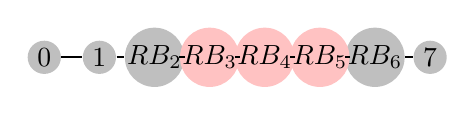
\begin{tikzpicture}[scale=0.7]
    % Draw a 7,11 network
    % First we draw the vertices
    \foreach \pos/\name in {{(0,1)/1},{(6,1)/7},{(1,1)/RB_2},{(5,1)/RB_6},{(-1,1)/0}}
        \node[vertex] (\name) at \pos {$\name$};
        
    \foreach \pos/\name in {{(2,1)/RB_3}, {(3,1)/RB_4}, {(4,1)/RB_5}}
    \node[selected vertex] (\name) at \pos {$\name$};
    
    % Connect vertices with edges 
    \foreach \source/ \dest in {1/RB_2,RB_2/RB_3, RB_3/RB_4, RB_4/RB_5, RB_5/RB_6,RB_6/7,0/1}
        \path[edge] (\source) -- (\dest) ;
        
\end{tikzpicture}
\end{center}

Then define \[\leq^1\] by
\[i\in \leq^1 \Leftrightarrow \exists  j\in \bar{G}_i (I^1_i\subseteq G^1_j\cap R^0)\] 

\begin{itemize}
\item For instance, \[3\in \leq^1, 4\notin \leq^0\]
\item Since 
\begin{table}[h]
\begin{tabular}{l l}
$I^1_3=\{2,3,4,5\}$ & $G^1_3\cap R^0=\{2,3,4,5\} $  \\
$I^1_4=\{2,3,4,5,6\}$ & $G^1_4\cap R^0=\{2,3,4,5,6\} $  \\
\end{tabular}
\end{table}
\end{itemize}



\end{frame}


\begin{frame}
  \frametitle{Information Hierarchy}


\begin{center}
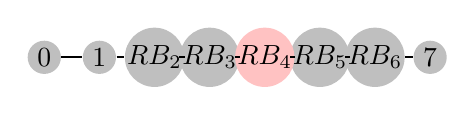
\begin{tikzpicture}[scale=0.7]
    % Draw a 7,11 network
    % First we draw the vertices
    \foreach \pos/\name in {{(0,1)/1},{(6,1)/7},{(1,1)/RB_2},{(5,1)/RB_6},{(2,1)/RB_3}, {(4,1)/RB_5},{(-1,1)/0}}
        \node[vertex] (\name) at \pos {$\name$};
        
    \foreach \pos/\name in { {(3,1)/RB_4}}
    \node[selected vertex] (\name) at \pos {$\name$};
    
    % Connect vertices with edges 
    \foreach \source/ \dest in {1/RB_2,RB_2/RB_3, RB_3/RB_4, RB_4/RB_5, RB_5/RB_6,RB_6/7,0/1}
        \path[edge] (\source) -- (\dest) ;
        
\end{tikzpicture}
\end{center}

At $\alert{2}$-block, let

\[
\alert{R^{2}} \equiv \{i\in R^1|i\notin \leq^1\}=\{\invisible{2,3,}4\invisible{,5,6}\}
\]



\end{frame}





\begin{frame}
  \frametitle{Information Hierarchy}


\begin{theorem}
\label{lemma_empty}
Given $\theta$, if
\begin{enumerate}
\item the network is FFCCU and acyclic
\item the state has strong connectedness
\end{enumerate}
$\Rightarrow$ $\exists t^{\theta}$ and $\exists i\in R^{t^{\theta}}$ such that $I^{t^{\theta}}_i \supset [Rebels](\theta) $.
\end{theorem} 

So, APEX can be attained by

\begin{table}[h]
\begin{tabular}{l l l l}
$R^t$ Rebels & play & $\langle I^{t-1}_i\rangle$ & $\textbf{s},...,\textbf{s},\overbrace{\textbf{r},\textbf{s},...,\textbf{s}}^{\prod_{j\in I^{t-1}_i}x_j}$ \\
\hline
non-$R^t$ Rebels & play & $\langle \textbf{stay} \rangle$ & $\textbf{s},...,\textbf{s},\textbf{s},\textbf{s},...,\textbf{s}$  \\

\end{tabular}
\end{table}

\alert{However, ``Pivotal Rebels'' will deviate}.


\end{frame}


\begin{frame}
  \frametitle{Information Hierarchy}

\textbf{Pivotal players}

\begin{definition}
$i$ is pivotal in $RP^t$ $\Leftrightarrow$ $i\in R^t$ and $i$ \textbf{will} know $\#[Rebels](\theta)\geq k$ or $\#[Rebels](\theta)< k$ after $RP^t$ \textbf{before} $I^{t-1}_i$ is reported.
\end{definition}

\begin{enumerate}
\item Ex. $k=5$
\item Rebel 4 and Rebel 5 are pivotal (\textbf{Free Rider problem})
\begin{center}
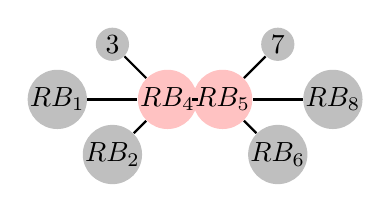
\begin{tikzpicture}[scale=0.7]
    % Draw a 7,11 network
    % First we draw the vertices
    \foreach \pos/\name in {{(1,2)/RB_1}, {(2,1)/RB_2}, {(2,3)/3}, {(5,1)/RB_6}, {(5,3)/7}, {(6,2)/RB_8}}
        \node[vertex] (\name) at \pos {$\name$};
    
    \foreach \pos/\name in {{(3,2)/RB_4}, {(4,2)/RB_5}}
    \node[selected vertex] (\name) at \pos {$\name$};
    
    % Connect vertices with edges 
    \foreach \source/ \dest in {RB_1/RB_4, RB_2/RB_4,3/RB_4,RB_4/RB_5, RB_5/RB_6, RB_5/7, RB_5/RB_8}
        \path[edge] (\source) -- (\dest) ;
        
\end{tikzpicture}
\end{center}

\item They will manipulate their reporting to save costs.
\begin{itemize}
\item By reporting some other number.
\end{itemize}
\end{enumerate}



\end{frame}



\begin{frame}
  \frametitle{Information Hierarchy}

\textbf{Pivotal players}

\begin{definition}
$i$ is pivotal in $RP^t$ $\Leftrightarrow$ $i\in R^t$ and $i$ \textbf{will} know that $\#[Rebels](\theta)\geq k$ or $\#[Rebels](\theta)< k$ after $RP^t$ \textbf{before} $I^{t-1}_i$ is reported.
\end{definition}

\begin{enumerate}
\item Ex. $k=6$
\item Rebel 4 is pivotal
\begin{center}
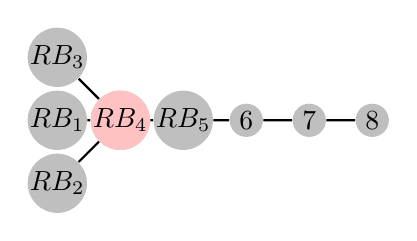
\begin{tikzpicture}[scale=0.8]
    % Draw a 7,11 network
    % First we draw the vertices
    \foreach \pos/\name in {{(2,2)/RB_1}, {(2,1)/RB_2}, {(2,3)/RB_3}, {(3,2)/RB_4}, {(4,2)/RB_5}, {(5,2)/6}, {(6,2)/7}, {(7,2)/8}}
        \node[vertex] (\name) at \pos {$\name$};
    
    \foreach \pos/\name in { {(3,2)/RB_4}}
    \node[selected vertex] (\name) at \pos {$\name$};
    
    % Connect vertices with edges 
    \foreach \source/ \dest in {RB_1/RB_4, RB_2/RB_4,RB_3/RB_4,RB_4/RB_5, RB_5/6, 6/7, 7/8}
        \path[edge] (\source) -- (\dest) ;
        
\end{tikzpicture}
\end{center}

\item He will manipulate his reporting to save costs.
\begin{itemize}
\item By reporting some other number.
\end{itemize}
\end{enumerate}



\end{frame}


\begin{frame}
  \frametitle{Information Hierarchy}

\textbf{Solving Pivotal-player problem. Step 1.}

\begin{definition}\textbf{Free Rider Problem}
A FRP in a $t$-block is that $\exists i,j\in R^t$, $i\neq j$ such that
\begin{enumerate}
\item $i,j$ is pivotal in $RP^t$
\item $i, j$ \textbf{will} know the $\#[Rebels](\theta)$ after $RP^t$ \textbf{before} $I^{t-1}_i$ is reported.
\end{enumerate}
\end{definition}



\end{frame}


\begin{frame}
  \frametitle{Information Hierarchy}

\textbf{Solving Pivotal-player problem. Step 1.}



\begin{lemma}
If networks are acyclic, then
\begin{itemize}
\item there is a \alert{unique block} $B^t$ where FRP may occur. 
\item there are only \alert{two} $i,j\in R^t$ are involved, and \alert{$i\in G_j$}.
\item Moreover, both of $i,j$ know that they will be involved \alert{before} $B^t$ and \alert{after} $B^{t-1}$.
\end{itemize}


\end{lemma}
Thus, {before} $B^t$ and {after} $B^{t-1}$, pick one of them be pivotal player.
\begin{itemize}
\item By their prim number.
\end{itemize} 


\end{frame}


\begin{frame}
  \frametitle{Information Hierarchy}

\textbf{Solving Pivotal-player problem. Step 2.}

\begin{table}[h]
\begin{tabular}{l l l l}
Non-pivotal $R^t$ Rebels & play & $\langle I^{t-1}_i\rangle$ & $\textbf{s},...,\textbf{s},\overbrace{\textbf{r},\textbf{s},...,\textbf{s}}^{\prod_{j\in I^{t-1}_i}x_j}$ \\
Pivotal $R^t$ Rebels & \alert{may} play & \alert{$\langle 1\rangle$} & $\textbf{s},...,\textbf{s},\textbf{s},\textbf{s},...,\alert{\textbf{r}}$ \\
\hline
non-$R^t$ Rebels & play & $\langle \textbf{stay} \rangle$ & $\textbf{s},...,\textbf{s},\textbf{s},\textbf{s},...,\textbf{s}$  \\

\end{tabular}
\end{table}

I.e. Add \alert{$\langle 1\rangle$} into the equilibrium path.

\end{frame}

\begin{frame}
  \frametitle{Information Hierarchy}

\textbf{Solving Pivotal-player problem. Step 3.}

In the equilibrium path,  
\begin{lemma}
If networks are acyclic, in $RP^t$, before $i$ plays $I^{t-1}_i$
\[ \text{$i$ knows that $\#[Rebels](\theta)\geq k-1$}\] $\Leftrightarrow$ \[\text{$i$ is pivotal but $i$ may not know $\#[Rebels](\theta)$ after $RP^t$}\]
\end{lemma}

\begin{lemma}
If networks are acyclic, 
\[ \text{$i$ knows that $\#[Rebels](\theta)\geq k-1$}\] $\Leftrightarrow$ \[\text{$i$ play $\langle 1 \rangle$}\]
\end{lemma}




\end{frame}


\begin{frame}
  \frametitle{Information Hierarchy}

\textbf{Solving Pivotal-player problem. Step 3.}

Consequently, in the path,

\begin{table}[h]
\begin{tabular}{l l l l}
$i$ has played  & $i$ in FRP & $j\in G_i$ play & $i$ knows \\
\hline
\hline
$\langle 1 \rangle$ & yes  & $\langle \cdot \rangle$ & $\#[Rebels](\theta)\geq k$ \\
$\langle 1 \rangle$&   no  & $\langle 1 \rangle$ & $\#[Rebels](\theta)\geq k$ \\
$\langle 1 \rangle$&   no  & $\langle \textbf{stay} \rangle$ & $\#[Rebels](\theta)< k$ \\

\end{tabular}
\end{table}

$i$ has to play \textbf{message to revolt} or \textbf{message to revolt} if he played $\langle 1 \rangle$

\begin{table}[ht]
\caption{Equilibrium path if $i$ played $\langle 1 \rangle$}
\label{Table_blf_up_cdt12}
\begin{center}
\begin{tabular}{l c c l}
In $RP^t$ 	 	&  	In $CD^t_{1,1}$		&  In $CD^t_{1,2}$	 & After \\
\hline
\hline
$i$ plays 		                             &  	$i$ plays		&				$i$ plays			& \\
\hline
$\langle 1 \rangle$ 		             &  \alert{$\langle \textbf{stay} \rangle$}	&	$\langle \textbf{stay} \rangle$ & \textbf{coordination to stay}\\
$\langle 1 \rangle$ 		             &  $\langle \mathbf{x}_i \rangle$	&	\alert{${\langle \textbf{stay} \rangle}$} & \textbf{coordination to revolt}\\
\end{tabular}
\end{center}
\end{table}
\end{frame}


\begin{frame}
\frametitle{Beliefs in equilibrium path}

\textbf{In the equilibrium path}

\begin{table}[h]
\caption{In $RP^t$}
\begin{tabular}{l l l l}
$R^t$ & either play & $\langle I^{t-1}_i\rangle$ & $\textbf{s},...,\textbf{s},\overbrace{\textbf{r},\textbf{s},...,\textbf{s}}^{\prod_{j\in I^{t-1}_i}x_j}$ \\
$R^t$ & or play &  {$\langle 1 \rangle$} & $\textbf{s},...,\textbf{s},\textbf{s},\textbf{s},...,\textbf{r}$  \\
\hline
$R^t$ & play & $\langle \textbf{stay} \rangle$ & $\textbf{s},...,\textbf{s},\textbf{s},\textbf{s},...,\textbf{s}$  \\

\end{tabular}
\end{table}


\begin{table}[ht]
\caption{Belief updating after $CD^t$, $t>0$}
\label{Table_blf_up_cdt12}
\begin{center}
\begin{tabular}{l c c c}
In $RP^t$ 	 	&  	In $CD^t_{1,1}$		&  In $CD^t_{1,2}$	  &\\
\hline
\hline
$i$ plays 		                             &  	$i$ plays		&				$i$ plays			& The events $j$ believe with probability one  \\
\hline
$\langle  \textbf{stay} \rangle$ 	& 	$\langle \mathbf{x}_i \rangle$	&  $\langle \textbf{stay} \rangle$ &  $i\notin R^t$ \\
$\langle  {I^{t-1}_i} \rangle$ 		&  $\langle \textbf{stay} \rangle$	&	$\langle \textbf{stay} \rangle$ &  $\#[Rebels](\theta)< k$   \\
$\langle  {I^{t-1}_i} \rangle$ 		&  $\langle \mathbf{x}_i \rangle$	&	$\langle \textbf{stay} \rangle$ &  $\#[Rebels](\theta)\geq k$    \\
$\langle  {I^{t-1}_i} \rangle$ 		&  $\langle \mathbf{x}_i \rangle$	&	$\langle \mathbf{x}_i \rangle$ &  $i\in R^t$  \\
$\langle 1 \rangle$ 		             &  $\langle \textbf{stay} \rangle$	&	$\langle \textbf{stay} \rangle$ &  $\#[Rebels](\theta)< k$\\
$\langle 1 \rangle$ 		             &  $\langle \mathbf{x}_i \rangle$	&	$\langle \textbf{stay} \rangle$ & $\#[Rebels](\theta)\geq k$
\end{tabular}
\end{center}
\end{table}

 
\end{frame}




\begin{frame}
\frametitle{Off-path Belief}

Whenever $i$ detects a deviation, he believes that
\[\text{for all $j\notin G_i$, $\theta_j\neq$Rebel  }\]

\begin{enumerate}
\item If $\# (G_i\cap [Rebels](\theta))<k$, he will play \textbf{stay} forever.
\item This off-path belief then also serve as a grim trigger - \alert{belief-grim-trigger}.
\end{enumerate}




\end{frame}


\begin{frame}
\frametitle{Sketch of proof}

\begin{enumerate}
\item The equilibrium path is APEX.
\item If game enters $B^t$, all Rebels have not know relevant info. before $B^t$.
\item Detectable deviation $\Rightarrow$ APEX \textbf{may} fail by belief-grim-trigger.
\item Undetectable deviation $\Rightarrow$ APEX \textbf{may} fail by protocol-grim-trigger
\begin{itemize}
\item pivotal $R^t$, non-pivotal $R^t$, non-$R^t$, will not mimic each other.
\end{itemize}
\item Ex-post outcome gives maximum ex-post static pay-off.
\item Sufficiently high $\delta$ will impede deviation.
\end{enumerate}



\end{frame}


\begin{frame}
\frametitle{Discussion}

\begin{enumerate}


\item From the above steps, an APEX equilibrium for acyclic networks is constructed.
\item Solving Pivotal-player problem for cyclic networks need more elaboration
\begin{center}
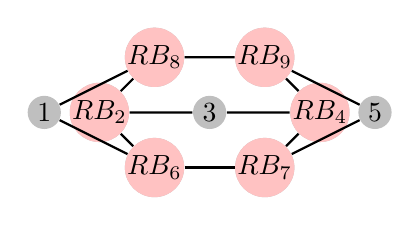
\begin{tikzpicture}[scale=0.7]
    % Draw a 7,11 network
    % First we draw the vertices
    \foreach \pos/\name in {{(1,3)/1}, {(2,3)/RB_2}, {(4,3)/3}, {(6,3)/RB_4}, {(7,3)/5}, {(3,2)/RB_6}, {(5,2)/RB_7}, {(3,4)/RB_8}, {(5,4)/RB_9}}
        \node[vertex] (\name) at \pos {$\name$};
    
    \foreach \pos/\name in {{(2,3)/RB_2},{(6,3)/RB_4},{(3,2)/RB_6}, {(5,2)/RB_7}, {(3,4)/RB_8}, {(5,4)/RB_9}}
    \node[selected vertex] (\name) at \pos {$\name$};
    
    % Connect vertices with edges 
    \foreach \source/ \dest in { 1/RB_6, 1/RB_8, RB_2/3, RB_2/RB_8, 3/RB_4, RB_2/RB_6, RB_6/RB_7, RB_8/RB_9, RB_9/RB_4, RB_7/RB_4, RB_9/5, RB_7/5}
        \path[edge] (\source) -- (\dest) ;
        
\end{tikzpicture}
\end{center}


\end{enumerate}


\end{frame}


\begin{frame}
\frametitle{Discussion}

\begin{enumerate}


\item From the above steps, an APEX equilibrium for acyclic networks is constructed.
\item Solving Pivotal-player problem for cyclic networks need more elaboration

\begin{center}
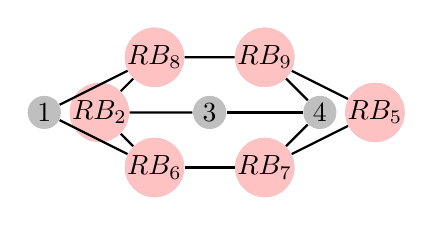
\begin{tikzpicture}[scale=0.7]
    % Draw a 7,11 network
    % First we draw the vertices
    \foreach \pos/\name in {{(1,3)/1}, {(2,3)/RB_2}, {(4,3)/3}, {(6,3)/4}, {(7,3)/RB_5}, {(3,2)/RB_6}, {(5,2)/RB_7}, {(3,4)/RB_8}, {(5,4)/RB_9}}
        \node[vertex] (\name) at \pos {$\name$};
    
    \foreach \pos/\name in {{(2,3)/RB_2},{(7,3)/RB_5},{(3,2)/RB_6}, {(5,2)/RB_7}, {(3,4)/RB_8}, {(5,4)/RB_9}}
    \node[selected vertex] (\name) at \pos {$\name$};
    
    % Connect vertices with edges 
    \foreach \source/ \dest in { 1/RB_6, 1/RB_8, RB_2/3, RB_2/RB_8, 3/4, RB_2/RB_6, RB_6/RB_7, RB_8/RB_9, RB_9/4, RB_7/4, RB_9/RB_5, RB_7/RB_5}
        \path[edge] (\source) -- (\dest) ;
        
\end{tikzpicture}
\end{center}

\end{enumerate}


\end{frame}


\begin{frame}
\frametitle{Discussion}

\begin{enumerate}

\item payoff is perfectly observed
\begin{itemize}
\item Play \textbf{revolt} in the first period, then the relevant information revealed.

\end{itemize}
\item payoff is noisy
\begin{itemize}
\item With full support assumption, the existing equilibrium is APEX.
\item Ex. 
\begin{eqnarray*}
p_{1s} &=& \mathrm {Pr}(y=y_1|\#\textbf{revolt}\geq k) \\
p_{1f} &=& \mathrm {Pr}(y=y_1|\#\textbf{revolt}< k) \\
p_{2s} &=& \mathrm {Pr}(y=y_2|\#\textbf{revolt}\geq k) \\
p_{2f} &=& \mathrm {Pr}(y=y_2|\#\textbf{revolt}< k) 
\end{eqnarray*}

\begin{equation}
1>p_{1s}>0,1>p_{2s}>0,p_{1f}=1-p_{1s},p_{2f}=1-p_{2s}
\end{equation}
\end{itemize}


\end{enumerate}


\end{frame}





\begin{frame}

\frametitle{Further works}


\begin{enumerate}
\item For the networks with circles, the proof for an APEX equilibrium is still open.
\item There should be a general model in which players can communicate only by their actions to learn the relevant information in finite time when $\delta<1$, while the communication protocol itself is an equilibrium.
\item Communication in network could serve as a criteria in equilibrium selection.  

\end{enumerate}
\end{frame}










\end{document}
